\documentclass[11pt]{beamer}
\usepackage[utf8]{inputenc}
\usepackage[T1,T2A]{fontenc}
\usepackage[russian]{babel}
\usepackage{color}
\usepackage{calc}
\usepackage{graphicx}
\usepackage{epstopdf}
\usepackage{hyperref}
\hypersetup{unicode,colorlinks}
\usetheme[progressbar=head,numbering=fraction,block=fill]{metropolis}
\usepackage{minted}
\usepackage{dejavu}
%\usepackage{adjustbox}  % Позволяет сузить куски кода (или текст) ровно настолько, чтобы уместиться в слайд
\usepackage{csquotes}
\usepackage{upquote}

\usemintedstyle{solarized-light}
\newminted[haskell]{haskell}{
    escapeinside=!!,
    mathescape=true,
    texcomments=true,
    beameroverlays=true,
    autogobble=true,
    fontsize=\small,
    breaklines=false  % Лучше сам поставлю переносы на удобных местах
}
\newminted[haskellsmall]{haskell}{
    escapeinside=!!,
    mathescape=true,
    texcomments=true,
    beameroverlays=true,
    autogobble=true,
    fontsize=\footnotesize,
    breaklines=false
}
\newminted[haskelltiny]{haskell}{
    escapeinside=!!,
    mathescape=true,
    texcomments=true,
    beameroverlays=true,
    autogobble=true,
    fontsize=\scriptsize,
    breaklines=false
}
\newmintinline[haskinline]{haskell}{
    escapeinside=!!,
    mathescape=true,
    beameroverlays=true,
    breaklines=true
}
\newminted[ghci]{text}{
    autogobble=true,
    fontsize=\small,
    breaklines=false
}
\newminted[ghcismall]{text}{
    autogobble=true,
    fontsize=\footnotesize,
    breaklines=false
}
\newminted[ghcitiny]{text}{
    autogobble=true,
    fontsize=\scriptsize,
    breaklines=false
}
\newmintinline[ghcinline]{text}{
    breaklines=true
}

\newcommand{\hackage}[1]{\href{https://hackage.haskell.org/package/#1}{#1}}

\vfuzz=20pt  % позволяет тексту дойти до номера слайда

\author{Алексей Романов}
\subtitle{Функциональное программирование на Haskell}
%\logo{}
\institute{МИЭТ}
\subject{Функциональное программирование на Haskell}
%\setbeamercovered{transparent}
%\setbeamertemplate{navigation symbols}{}


\title{Лекция 9: функторы, монады и все-все-все}

\begin{document}
\begin{frame}[plain]
  \maketitle
\end{frame}

\begin{frame}[fragile]
  \frametitle{Роды типов}
  \begin{itemize}
    \item У значений есть типы, а у типов "--- р\'{о}ды (kinds).
    \item Все обычные типы (\haskinline|Int|, \haskinline|Maybe Bool|, \haskinline|(Int, Int)|, \ldots) имеют род \haskinline|*| (синоним "--- \haskinline|Type|).
          \pause
    \item Пример более сложного рода "--- \haskinline|Maybe|. Он принимает тип рода \haskinline|*| и возвращает тип рода \haskinline|*|:
          \begin{haskell}
            ghci> :kind Maybe !\pause!
            Maybe :: * -> *
          \end{haskell}
          \pause
    \item Определите род:
          \begin{itemize}
            \item \haskinline!Either! (\haskinline!data Either a b = Left a | Right b!)
                  \pause
            \item \haskinline!Shape! (\haskinline|type Shape f = f ()|)
                  \pause
          \end{itemize}
    \item В стандартном Haskell все роды строятся из \haskinline|*| и \haskinline|->|, в GHC всё сложнее (\href{https://downloads.haskell.org/~ghc/8.6.3/docs/html/users_guide/glasgow_exts.html#kind-polymorphism}{Kind polymorphism}, \href{https://downloads.haskell.org/~ghc/8.6.3/docs/html/users_guide/glasgow_exts.html#unboxed-types-and-primitive-operations}{Unboxed type kinds}, \href{https://downloads.haskell.org/~ghc/8.6.3/docs/html/users_guide/glasgow_exts.html#datatype-promotion}{Datatype promotion},  \href{https://downloads.haskell.org/~ghc/8.6.3/docs/html/users_guide/glasgow_exts.html#the-constraint-kind}{The \haskinline|Constraint| kind}).
  \end{itemize}
\end{frame}

\begin{frame}[fragile]
  \frametitle{Частичное применение типов}
  \begin{itemize}
    \item Конструкторы типов могут быть частично применены (как функции).
    \item Если \haskinline!Either :: * -> * -> *!, то \haskinline|Either Int|\pause\haskinline| :: * -> *|. \haskinline|Either a| "--- тоже.
          \pause
    \item Типы кортежей, функций и списков можно писать в префиксном виде: \\
          \haskinline|(,) a b|, \haskinline|(->) a b|, \haskinline|[] a|.
          \pause
    \item И применять частично: \haskinline|(->) Int| читается как \enquote{функции из \haskinline|Int|} и имеет род \pause\haskinline|* -> *|.
          \pause
    \item Синонимы типов (как \haskinline|Shape| с прошлого слайда) всегда должны быть применены полностью.
          \pause
    \item Для частичного применения нужен \\
          \haskinline|newtype Shape f = Shape (f ())|.
  \end{itemize}
\end{frame}

\begin{frame}[fragile]
  \frametitle{Варианты \haskinline|map|}
  \begin{itemize}
    \item Сравним типы нескольких функций:
    \item \alt<-4>{\haskinline|map :: (a -> b) -> [a] -> [b]|}{\haskinline|map :: (a -> b) -> [] a -> [] b|}
          \pause
    \item \haskinline|mapMb :: (a -> b) -> Maybe a -> Maybe b| (\haskinline|mapMaybe| называется другая функция)
          \pause
    \item \haskinline|mapMap :: (a -> b) -> Map k a -> Map k b| (она же \haskinline|Data.Map.{Lazy/Strict}.map|)
          \pause
    \item \alt<+>{\haskinline|mapSnd :: (a -> b) -> (c, a) -> (c, b)|}{\haskinline|mapSnd :: (a -> b) -> (,) c a -> (,) c b|} \pause
    \item Видим, что все они имеют вид \pause \\
          \haskinline|forall a b. (a -> b) -> f a -> f b| для разных \haskinline|f| (\haskinline|f| не под \haskinline|forall|!).
  \end{itemize}
\end{frame}

\begin{frame}[fragile]
  \frametitle{Функторы}
  \begin{itemize}
    \item Можем обобщить все функции с предыдущего слайда, введя класс типов
          \begin{haskell}
            class Functor f where
              fmap :: (a -> b) -> f a -> f b
              (<$) :: a        -> f b -> f a
              (<$) = fmap . const
          \end{haskell}
    \item Здесь \haskinline|f| "--- переменная типа сорта \pause \haskinline|* -> *|.
    \item Смысл \haskinline|fmap g xs|: применить функцию \haskinline|g| ко всем значениям типа \haskinline|a| \enquote{внутри} \haskinline|xs|, не меняя структуры.
    \item \haskinline|(<$)| "--- частный случай \haskinline|fmap|, который иногда может быть реализован напрямую.
          \pause
    \item \haskinline|(<$>)| "--- синоним \haskinline|fmap| как оператор.
  \end{itemize}
\end{frame}

\begin{frame}[fragile]
  \frametitle{Законы функторов}
  \begin{itemize}
    \item Что значит \enquote{не меняя структуры}?
    \item Например, рассмотрим случай \haskinline|fmap id|. Чему должно быть равно \haskinline|fmap id xs|? \pause
          \begin{haskell}
fmap id xs == xs
\end{haskell}
          \pause
    \item Этот закон также формулируется как \\ \alt<+>{\haskinline|fmap id == id|}{\haskinline|fmap (id @a) == id @(f a)|}. \pause
    \item Второй закон функторов:
          \begin{haskell}
            fmap (g . h) xs ==!\pause! fmap g (fmap h xs)
          \end{haskell}
          \pause
          \begin{haskell}
fmap (g . h)    ==!\pause! fmap g . fmap h
\end{haskell}
  \end{itemize}
\end{frame}

\begin{frame}[fragile]
  \frametitle{Примеры функторов}
  \begin{itemize}
    \item Очень многие типы (рода \haskinline|* -> *|) являются функторами. Например:
          \begin{haskell}
            instance Functor Maybe where 
              -- fmap :: (a -> b) -> Maybe a -> Maybe b
              fmap f (Just x) =!\pause! Just (f x)
              fmap _ Nothing  =!\pause! Nothing
          \end{haskell}
          \pause
    \item
          \begin{haskell}
            instance Functor [] where 
              fmap =!\pause! map
          \end{haskell}
    \item Не можем определить
          \begin{haskell}
            instance Functor [] where 
              fmap f xs = []
          \end{haskell}
          \pause
          Типы сходятся (проверьте!), но законы нарушены.
  \end{itemize}
\end{frame}

\begin{frame}[fragile]
  \frametitle{Ещё примеры функторов}
  \begin{itemize}
    \item Частично применённые кортежи:
          \begin{haskell}
            instance Functor ((,) c) where 
            -- fmap :: (a -> b) -> (c, a) -> (c, b)
            fmap f (z, x) =!\pause! (z, f x)
          \end{haskell}
          \pause
    \item
          \begin{haskell}
            data Pair a = Pair a a
            instance Functor Pair where 
            -- fmap :: (a -> b) -> Pair a -> Pair b
            fmap f (Pair x y) =!\pause! Pair (f x) (f y)
          \end{haskell}
          \pause
    \item Дома (начните с уточнения типа \haskinline|fmap|):
          \begin{haskell}
            instance Functor (Either c) where ...
            instance Functor ((->) c) where ...
          \end{haskell}
  \end{itemize}
\end{frame}

\begin{frame}[fragile]
  \frametitle{... и нефункторов}
  \begin{itemize}
    \item Не все типы можно сделать функторами! Рассмотрим
          \begin{haskell}
            newtype Pred a = Pred (a -> Bool)
            instance Functor Pred where 
            -- fmap :: (a -> b) -> Pred a -> Pred b
            fmap g (Pred p) =!\pause! Pred (\x -> ???)
          \end{haskell}
          \pause \haskinline|g :: a -> b| не к чему применить: у нас нет ничего типа \haskinline|a|!
          \pause
    \item Общее правило: \haskinline|instance Functor F| можно определить, если \haskinline|a| не входит в определение \haskinline|F a| слева от нечётного числа \haskinline|->| (\href{https://downloads.haskell.org/~ghc/8.6.3/docs/html/users_guide/glasgow_exts.html#deriving-functor-instances}{объяснение}).
          \pause
    \item По этому правилу, функтор ли ниже?
          \begin{haskell}
            newtype Tricky a = T ((a -> Int) -> a)
          \end{haskell}
  \end{itemize}
\end{frame}

\begin{frame}[fragile]
  \frametitle{Доказательство законов для экземпляра \haskinline|Functor|}
  \begin{itemize}
    \item Возьмём для примера \haskinline|instance Functor Pair|. Нужно доказать, что для него:
    \item $\forall$ \haskinline|a :: *|, \haskinline|pair :: Pair a|
          \begin{haskell}
            fmap id pair == pair
          \end{haskell}
          \pause
    \item Шаг 1: \haskinline|pair = Pair x y|, где \haskinline|x, y :: |\pause\haskinline|a|
          \begin{haskell}
            fmap id pair ==
            fmap id (Pair x y) == !\pause! -- определение fmap \pause
            Pair (id x) (id y) == !\pause! -- определение id \pause
            Pair x y == 
            pair
          \end{haskell}
          \pause
    \item $\forall$ \haskinline|a, b, c :: *|, \haskinline|pair :: Pair a|, \haskinline|h :: a -> b|, \haskinline|g :: b -> c|
          \begin{haskell}
            fmap (g . h) pair == fmap g (fmap h pair)
          \end{haskell}
  \end{itemize}
\end{frame}

\begin{frame}[fragile]
  \frametitle{Использование функторов}
  \begin{itemize}
    \item Предскажите результаты:
          \begin{haskell}
            (+ 3) <$> Just 1
            (+ 3) <$> Nothing
            (+ 3) <$> [1, 2, 3]
          \end{haskell}
          \pause
    \item[]
    \item
          \begin{haskell}
            void :: Functor f => f a -> f ()
            void x = ???

            void [1, 2]
          \end{haskell}
  \end{itemize}
\end{frame}

\begin{frame}[fragile]
  \frametitle{Чего не могут функторы?}
  \begin{itemize}
    \item Удобно считать, что \haskinline|fmap| берёт функцию \haskinline|a -> b| и \enquote{поднимает} её в тип \haskinline|f a -> f b|.
    \item Можно ли с её помощью поднять функцию двух аргументов? Т.е. можно ли реализовать
          \begin{haskellsmall}
            fmap2 :: Functor f => (a -> b -> c) -> f a -> f b -> f c
            fmap2 g fx fy = ???
          \end{haskellsmall}
          \pause
    \item Нет! Единственное, с чего мы можем начать: \pause \haskinline|fmap g|. Она имеет тип \pause \haskinline|f a -> f (b -> c)|.
    \item Применив к \haskinline|fx| (тип подходит), получим
          \haskinline|fmap g fx :: f (b -> c)|. \pause
    \item Но \haskinline|f (b -> c)| и  \haskinline|f b| скомбинировать уже не получится.
  \end{itemize}
\end{frame}

\begin{frame}[fragile]
  \frametitle{Аппликативные функторы}
  \begin{itemize}
    \item Если добавить к функторам метод получения \haskinline|f c| из \haskinline|f (b -> c)| и \haskinline|f b|, и метод поднятия любого значения, получится понятие аппликативного функтора:
          \begin{haskell}
            class Functor f => Applicative f where
              pure  :: a -> f a
              infixl 4 <*>, *>, <*
              (<*>) :: f (a -> b) -> f a -> f b
              (*>) :: f a -> f b -> f b
              (<*) :: f a -> f b -> f a
          \end{haskell}
    \item \haskinline|(*>)| и \haskinline|(<*)| имеют определения по умолчанию.
    \item Теперь можно определить
          \begin{haskell}
            liftA2 :: Applicative f => (a -> b -> c) -> 
              f a -> f b -> f c
            liftA2 g fx fy = ???
          \end{haskell}
  \end{itemize}
\end{frame}

\begin{frame}[fragile]
  \frametitle{Законы аппликативных функторов}
  \begin{itemize}
    \item У \haskinline|Applicative| 5 законов:
    \item
          \begin{haskell}
            pure id <*> v = v

            pure f <*> pure x = pure (f x)

            u <*> pure y = pure ($ y) <*> u

            u <*> (v <*> w) = pure (.) <*> u <*> v <*> w

            fmap g x = pure g <*> x
          \end{haskell}
  \end{itemize}
\end{frame}

\begin{frame}[fragile]
  \frametitle{Моноидальные функторы}
  \begin{itemize}
    \item Эти законы не очень удобны и их трудно запомнить. Но мы можем использовать другой класс:
    \item
          \begin{haskell}
            class Functor f => Monoidal f where
              unit :: f ()
              (**) :: f a -> f b -> f (a,b)
          \end{haskell}
    \item Он взаимовыразим с аппликативными функторами (т.е. \haskinline|pure| и \haskinline|(<*>)| выражаются через \haskinline|unit| и \haskinline|(**)| и наоборот).
    \item Законы ($\simeq$: с точностью до изоморфизма):
          \begin{haskell}
            unit ** v !$\simeq$! v
            u ** unit !$\simeq$! u
            u ** (v ** w) !$\simeq$! (u ** v) ** w
          \end{haskell}
    \item Упражнение: записать точные их версии
  \end{itemize}
\end{frame}

\begin{frame}[fragile]
  \frametitle{Примеры аппликативных функторов}
  \begin{itemize}
    \item Многие функторы являются аппликативными:
          \begin{haskell}
            instance Applicative Maybe where
              -- pure :: a -> Maybe a
              pure =!\pause! Just
              -- (<*>) :: Maybe (a -> b) -> Maybe a -> Maybe b
              Just g <*> Just x  =!\pause! Just (g x)
              _      <*> _       =!\pause! Nothing
          \end{haskell}
          \pause
    \item Для списков есть 2 варианта. Стандартный:
          \begin{haskell}
            instance Applicative [] where 
              -- pure :: a -> [a]
              pure x =!\pause! [x]
              -- (<*>) :: [a -> b] -> [a] -> [b]
              gs <*> xs =!\pause! [g x | g <- gs, x <- xs]
          \end{haskell}
  \end{itemize}
\end{frame}

\begin{frame}[fragile]
  \frametitle{Примеры аппликативных функторов}
  \begin{itemize}
    \item Второй аппликативный функтор для списков (определён в \haskinline|Control.Applicative|):
          \begin{haskell}
            newtype ZipList a = ZipList { getZipList :: [a] }
            instance Applicative ZipList where 
              (ZipList fs) <*> (ZipList xs) = ZipList (zipWith ($) fs xs)
              pure x = ???
          \end{haskell}
          \pause
    \item Подсказка: реализация определяется законом
          \begin{haskell}
            pure id <*> v = v
          \end{haskell}
          \pause
    \item Ответ:
          \begin{haskell}
            pure x = ZipList (repeat x)
          \end{haskell}
  \end{itemize}
\end{frame}

\begin{frame}[fragile]
  \frametitle{Пример неаппликативного функтора}
  \begin{itemize}
    \item
          \begin{haskell}
            instance Applicative ((,) c) where 
              -- pure :: a -> (c, a)
              pure = ???
          \end{haskell}
          \pause Невозможно определить без ограничений на \haskinline|c|.
          \pause
    \item А какие ограничения нужны? \pause
          \begin{haskell}
            instance Monoid c => Applicative ((,) c) where
              pure x = (mempty, x)
              (c1, g) <*> (c2, x) =!\pause! (c1 <> c2, g x)
          \end{haskell}
  \end{itemize}
\end{frame}

\begin{frame}[fragile]
  \frametitle{Что можно сделать с аппликативными функторами}
  \begin{itemize}
    \item Предскажите результаты:
          \begin{haskell}
            pure (+) <*> [2, 3, 4] <*> pure 4
            [(+1), (*2)] <*> [2, 3]
            [1, 2] *> [3, 4, 5]
            [1, 2] <* [3, 4, 5]
            ZipList [1, 2] *> ZipList [3, 4, 5]
          \end{haskell}
          \pause
    \item Реализуйте
          \begin{haskell}
            when :: Applicative f => Bool -> f () -> f ()    
            sequenceAL :: Applicative f => [f a] -> f [a]
          \end{haskell}
    \item У второй есть обобщённая версия \href{http://hackage.haskell.org/package/base/docs/Data-Traversable.html#v:sequenceA}{\haskinline|sequenceA|}, определяющая ещё один класс \haskinline|Traversable|.
  \end{itemize}
\end{frame}

\begin{frame}[fragile]
  \frametitle{... и что нельзя}
  \begin{itemize}
    \item Структура результата аппликативного вычисления зависит только от структуры аргументов, а не от значений внутри них.
    \item Т.е. мы не можем определить функцию
          \begin{haskell}
            ifA :: Applicative f => f Bool -> f a -> f a -> f a
          \end{haskell}
          так, чтобы выполнялось
          \begin{haskell}
            ifA [True]  [1, 2] [3] == [1, 2]
            ifA [False] [1, 2] [3] == [3]
          \end{haskell}
          (в случае списков структура "--- число элементов).
          \pause
    \item Попробуйте написать какие-нибудь варианты \haskinline|ifA| по типу и убедиться в этом.
          \pause
    \item Эту проблему решают монады, о которых будет следующая лекция.
  \end{itemize}
\end{frame}

\begin{frame}[fragile]
  \frametitle{Диаграмма классов типов высших родов}
  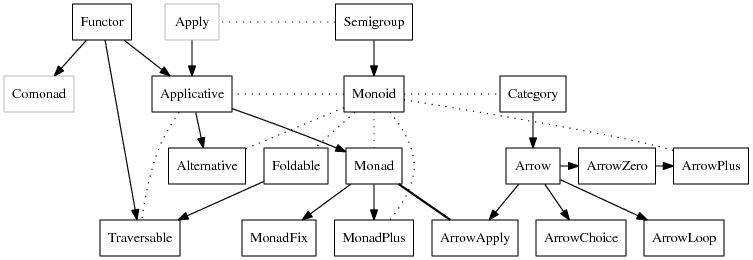
\includegraphics[width=\linewidth]{Typeclassopedia-diagram.png}
\end{frame}

% TODO восстановить слайды
%\begin{frame}[fragile]
%\frametitle{\haskinline|Foldable| и \haskinline|Traversable|}
%\begin{itemize}
%    \item TODO
%\end{itemize}
%\end{frame}
%
%\begin{frame}[fragile]
%\frametitle{Вывод \haskinline|Functor|, \haskinline|Foldable|, \haskinline|Traversable|}
%\begin{itemize}
%    \item TODO
%\end{itemize}
%\end{frame}

\begin{frame}[fragile]
  \frametitle{Дополнительное чтение}
  \begin{itemize}
    \item \href{https://wiki.haskell.org/Typeclassopedia}{Typeclassopedia} (диаграмма на предыдущем слайде оттуда). Особенно посмотрите на \haskinline|Foldable|, \haskinline|Traversable| и \haskinline|Alternative|.
    \item \href{https://stackoverflow.com/questions/7220436/good-examples-of-not-a-functor-functor-applicative-monad}{Good examples of Not a Functor/Applicative/Monad?}
    \item     \href{http://adit.io/posts/2013-04-17-functors,_applicatives,_and_monads_in_pictures.html}{Functors, Applicatives, And Monads In Pictures.}
    \item Глава \href{https://en.wikibooks.org/wiki/Haskell/Applicative_functors}{Applicative Functors} в Wikibook.
  \end{itemize}
\end{frame}

\end{document}
